% ============================================================
% CHAPTER 4: Sprint 5 & Sprint 6 — Quotas & Payments
% ============================================================
% ADD THIS TO main.tex AFTER COMPLETING SPRINT 5 & 6
% Uncomment: % ============================================================
% CHAPTER 4: Sprint 5 & Sprint 6 — Quotas & Payments
% ============================================================
% ADD THIS TO main.tex AFTER COMPLETING SPRINT 5 & 6
% Uncomment: % ============================================================
% CHAPTER 4: Sprint 5 & Sprint 6 — Quotas & Payments
% ============================================================
% ADD THIS TO main.tex AFTER COMPLETING SPRINT 5 & 6
% Uncomment: % ============================================================
% CHAPTER 4: Sprint 5 & Sprint 6 — Quotas & Payments
% ============================================================
% ADD THIS TO main.tex AFTER COMPLETING SPRINT 5 & 6
% Uncomment: \input{chapters/chapter4}
% ============================================================
\chapter{Sprint 5 \& Sprint 6: Quotas and Payment Service}

\section{Introduction}

This chapter covers the business logic layer of the platform. Sprint 5 implements the VM dashboard with detailed information and the quota system that enforces resource limits per user. Sprint 6 delivers the payment service with plan management and upgrade flows.

% ============================================================
% SPRINT 5
% ============================================================
\section{Sprint 5: VM Dashboard \& Quota System}

\sprintcard{5}{VM Dashboard \& Quota System}{Deliver a comprehensive VM dashboard with status monitoring, and implement quota enforcement to limit resource usage per plan.}

\subsection{Sprint Backlog}

\begin{longtable}{|c|p{5cm}|c|c|c|}
\hline
\rowcolor{blue!15}
\textbf{Task ID} & \textbf{Task} & \textbf{Assignee} & \textbf{Est.} & \textbf{Status} \\
\hline
\endhead
T-5.1 & VM detail page (frontend) & DSI & 5h & Done \\
\hline
T-5.10 & Web terminal (xterm.js + WebSocket SSH) & DSI & 6h & Done \\
\hline
T-5.2 & VM action buttons + confirmation & DSI & 4h & Done \\
\hline
T-5.3 & Quota tracking implementation & DSI & 4h & Done \\
\hline
T-5.4 & Quota enforcement on VM creation & DSI & 3h & Done \\
\hline
T-5.5 & Admin VM management page & DSI & 5h & Done \\
\hline
T-5.6 & Quota display on dashboard & DSI & 3h & Done \\
\hline
T-5.7 & Server monitoring setup & RSI & 6h & Done \\
\hline
T-5.8 & Backup procedures & RSI & 4h & Done \\
\hline
T-5.9 & Network security audit & RSI & 4h & Done \\
\hline
\caption{Sprint 5 backlog}
\label{tab:sprint5-backlog}
\end{longtable}

\subsection{Use Case Diagram — Quota Management}

\begin{figure}[H]
\centering
\begin{tikzpicture}[
  usecase/.style={draw, ellipse, minimum width=3cm, minimum height=0.8cm, align=center, font=\scriptsize}
]
  \draw[thick, rounded corners] (0, -4.5) rectangle (7, 0.5);
  \node[font=\small\bfseries] at (3.5, 0.2) {Quota Management};
  
  \node (user) at (-2, -1.5) {User};
  \node (system) at (9.5, -2) {System};
  
  \node[usecase] (uc1) at (3.5, -0.5) {View Quota Usage};
  \node[usecase] (uc2) at (3.5, -1.5) {View Plan Details};
  \node[usecase] (uc3) at (3.5, -2.5) {Request VM Creation};
  \node[usecase] (uc4) at (3.5, -3.5) {Check Quota Limit};
  
  \draw (user) -- (uc1);
  \draw (user) -- (uc2);
  \draw (user) -- (uc3);
  \draw[dashed] (uc3) -- node[right, font=\tiny] {<<include>>} (uc4);
  \draw (system) -- (uc4);
\end{tikzpicture}
\caption{Use case diagram — Quota management}
\label{fig:uc-quota}
\end{figure}

\subsection{Sequence Diagram — Quota Check on VM Creation}

\begin{figure}[H]
\centering
\begin{tikzpicture}[font=\small]
  \node (user) at (0, 0) {\textbf{User}};
  \node (vmsvc) at (4, 0) {\textbf{VM Service}};
  \node (quota) at (8, 0) {\textbf{Quota Service}};
  \node (db) at (12, 0) {\textbf{Database}};
  
  \draw[dashed] (user) -- (0, -8);
  \draw[dashed] (vmsvc) -- (4, -8);
  \draw[dashed] (quota) -- (8, -8);
  \draw[dashed] (db) -- (12, -8);
  
  \draw[->, thick] (0, -1) -- node[above, font=\tiny] {Create VM request} (4, -1);
  \draw[->, thick] (4, -2) -- node[above, font=\tiny] {Check user quota} (8, -2);
  \draw[->, thick] (8, -3) -- node[above, font=\tiny] {Get user plan + VM count} (12, -3);
  \draw[<-, thick] (8, -3.5) -- node[above, font=\tiny] {Plan: Pro, VMs: 3/5} (12, -3.5);
  \draw[<-, thick] (4, -4.5) -- node[above, font=\tiny] {Quota OK (3 < 5)} (8, -4.5);
  \draw[->, thick] (4, -5.5) -- node[right, font=\tiny] {Proceed with creation};
  
  % Alternative (quota exceeded)
  \draw[thick, red, dashed] (1, -6) rectangle (11, -7.5);
  \node[red, font=\tiny] at (6, -6.3) {alt: Quota Exceeded};
  \draw[->, thick, red] (8, -7) -- node[above, font=\tiny, red] {403 Quota Exceeded} (4, -7);
\end{tikzpicture}
\caption{Sequence diagram — Quota check on VM creation}
\label{fig:seq-quota}
\end{figure}

\subsection{Class Diagram — Quota \& Plan}

\begin{figure}[H]
\centering
\begin{tikzpicture}[font=\small,
  class/.style={draw, rectangle, minimum width=3.5cm, align=left}
]
  \node[class, fill=yellow!15] (plan) at (0, 0) {
    \textbf{Plan}\\
    \hline
    - id: UUID\\
    - name: String\\
    - maxVMs: Integer\\
    - maxCPU: Integer\\
    - maxRAM: Integer\\
    - maxDisk: Integer\\
    - price: Decimal\\
    \hline
    + getPlans()
  };
  
  \node[class, fill=blue!15] (quota) at (6, 0) {
    \textbf{UserQuota}\\
    \hline
    - id: UUID\\
    - userId: UUID\\
    - planId: UUID\\
    - usedVMs: Integer\\
    - usedCPU: Integer\\
    - usedRAM: Integer\\
    - usedDisk: Integer\\
    \hline
    + checkLimit()\\
    + updateUsage()
  };
  
  \draw[->, thick] (quota) -- node[above, font=\tiny] {belongs to} (plan);
\end{tikzpicture}
\caption{Class diagram — Plan and quota}
\label{fig:class-quota}
\end{figure}

\subsection{Implementation Screenshots}

\begin{figure}[H]
\centering
\fbox{\parbox{0.9\textwidth}{\centering\vspace{3cm}\textit{Insert VM detail page screenshot}\vspace{3cm}}}
\caption{VM detail page with status, IP, and resources}
\label{fig:vm-detail}
\end{figure}

\begin{figure}[H]
\centering
\fbox{\parbox{0.9\textwidth}{\centering\vspace{3cm}\textit{Insert quota usage display screenshot}\vspace{3cm}}}
\caption{Dashboard — Quota usage display}
\label{fig:quota-display}
\end{figure}
\subsection{Sequence Diagram --- Web Terminal Connection}

\begin{figure}[H]
\centering
\begin{tikzpicture}[font=\small]
  \node (user) at (0, 0) {\textbf{User}};
  \node (front) at (3, 0) {\textbf{Frontend}};
  \node (gate) at (6, 0) {\textbf{Gateway}};
  \node (proxy) at (9, 0) {\textbf{SSH Proxy}};
  \node (vm) at (12, 0) {\textbf{VM (SSH)}};
  
  \draw[dashed] (user) -- (0, -9);
  \draw[dashed] (front) -- (3, -9);
  \draw[dashed] (gate) -- (6, -9);
  \draw[dashed] (proxy) -- (9, -9);
  \draw[dashed] (vm) -- (12, -9);
  
  \draw[->, thick] (0, -0.8) -- node[above, font=\tiny] {Click ``Terminal''} (3, -0.8);
  \draw[->, thick] (3, -1.5) -- node[above, font=\tiny] {WebSocket connect} (6, -1.5);
  \draw[->, thick] (6, -2.2) -- node[above, font=\tiny] {Get user SSH key} (6, -2.2);
  \draw[->, thick] (6, -2.7) -- node[right, font=\tiny] {Verify JWT};
  \draw[->, thick] (6, -3.5) -- node[above, font=\tiny] {Open SSH tunnel} (9, -3.5);
  \draw[->, thick] (9, -4.2) -- node[above, font=\tiny] {SSH connect (key auth)} (12, -4.2);
  \draw[<-, thick] (9, -4.9) -- node[above, font=\tiny] {Shell session open} (12, -4.9);
  \draw[<-, thick] (6, -5.6) -- node[above, font=\tiny] {Tunnel ready} (9, -5.6);
  \draw[<-, thick] (3, -6.3) -- node[above, font=\tiny] {WS connected} (6, -6.3);
  \draw[->, thick] (3, -7) -- node[below, font=\tiny] {xterm.js renders terminal} (3, -7);
  \draw[<->, thick] (0, -7.5) -- node[above, font=\tiny] {Type commands / see output} (3, -7.5);
  \draw[<->, thick, blue, dashed] (3, -8.2) -- node[above, font=\tiny, blue] {Bidirectional data stream} (12, -8.2);
\end{tikzpicture}
\caption{Sequence diagram --- Web terminal connection (Phase~1)}
\label{fig:seq-terminal}
\end{figure}

\begin{figure}[H]
\centering
\fbox{\parbox{0.9\textwidth}{\centering\vspace{3cm}\textit{Insert web terminal (CLI) screenshot --- user accessing VM from browser}\vspace{3cm}}}
\caption{Web terminal --- CLI access to VM via xterm.js (Phase~1)}
\label{fig:web-terminal}
\end{figure}
\subsection{Sprint 5 Review}

At the end of Sprint 5:
\begin{itemize}
  \item VM detail page showing IP, status, OS, CPU, RAM, uptime.
  \item \textbf{Web terminal (Phase~1)} --- users can access VMs via a CLI terminal in the browser using xterm.js and WebSocket SSH proxy.
  \item VM action buttons (start, stop, reboot, delete) with confirmation dialogs.
  \item Quota system tracking and enforcing resource limits.
  \item Admin VM management page with filtering.
  \item Server monitoring and backup procedures in place.
\end{itemize}


% ============================================================
% SPRINT 6
% ============================================================
\section{Sprint 6: Payment Service}

\sprintcard{6}{Payment Service}{Implement payment processing with plan management, upgrade flows, and billing history.}

\subsection{Sprint Backlog}

\begin{longtable}{|c|p{5cm}|c|c|c|}
\hline
\rowcolor{blue!15}
\textbf{Task ID} & \textbf{Task} & \textbf{Assignee} & \textbf{Est.} & \textbf{Status} \\
\hline
\endhead
T-6.1 & Plans CRUD (backend) & DSI & 4h & Done \\
\hline
T-6.2 & Payment processing (Stripe/mock) & DSI & 5h & Done \\
\hline
T-6.3 & Billing page (frontend) & DSI & 4h & Done \\
\hline
T-6.4 & Checkout flow (frontend) & DSI & 5h & Done \\
\hline
T-6.5 & Payment history page & DSI & 3h & Done \\
\hline
T-6.6 & Admin plan management page & DSI & 3h & Done \\
\hline
T-6.7 & SSL/TLS configuration & RSI & 4h & Done \\
\hline
T-6.8 & Log management & RSI & 4h & Done \\
\hline
T-6.9 & OpenNebula optimization & RSI & 4h & Done \\
\hline
\caption{Sprint 6 backlog}
\label{tab:sprint6-backlog}
\end{longtable}

\subsection{Use Case Diagram — Payment}

\begin{figure}[H]
\centering
\begin{tikzpicture}[
  usecase/.style={draw, ellipse, minimum width=3cm, minimum height=0.8cm, align=center, font=\scriptsize}
]
  \draw[thick, rounded corners] (0, -5.5) rectangle (7, 0.5);
  \node[font=\small\bfseries] at (3.5, 0.2) {Payment Module};
  
  \node (user) at (-2, -2) {User};
  \node (admin) at (9.5, -4) {Admin};
  
  \node[usecase] (uc1) at (3.5, -0.5) {View Current Plan};
  \node[usecase] (uc2) at (3.5, -1.5) {Compare Plans};
  \node[usecase] (uc3) at (3.5, -2.5) {Upgrade Plan};
  \node[usecase] (uc4) at (3.5, -3.5) {Process Payment};
  \node[usecase] (uc5) at (3.5, -4.5) {View Payment History};
  
  \draw (user) -- (uc1);
  \draw (user) -- (uc2);
  \draw (user) -- (uc3);
  \draw (user) -- (uc5);
  \draw[dashed] (uc3) -- node[right, font=\tiny] {<<include>>} (uc4);
  
  \node[usecase] (uc6) at (7.5, -5) {Manage Plans (CRUD)};
  \draw (admin) -- (uc6);
\end{tikzpicture}
\caption{Use case diagram — Payment module}
\label{fig:uc-payment}
\end{figure}

\subsection{Sequence Diagram — Plan Upgrade}

\begin{figure}[H]
\centering
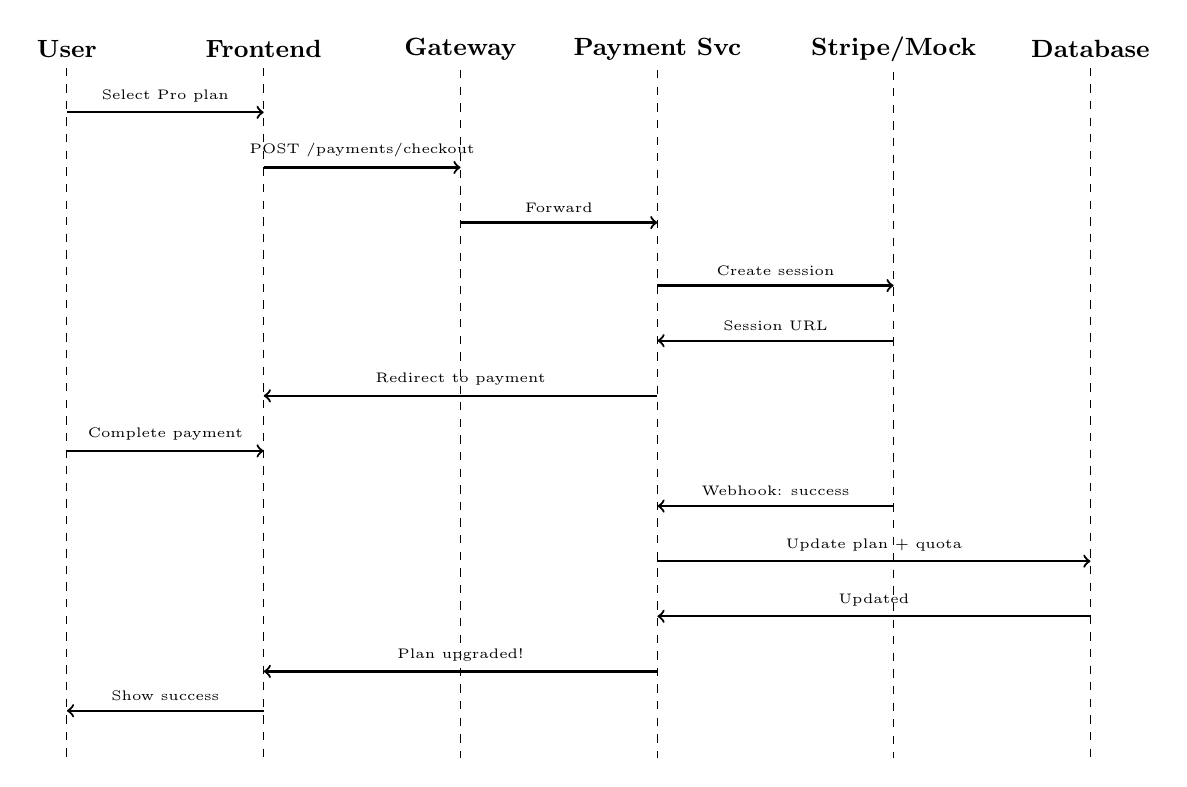
\begin{tikzpicture}[font=\small]
  \node (user) at (0, 0) {\textbf{User}};
  \node (front) at (2.5, 0) {\textbf{Frontend}};
  \node (gate) at (5, 0) {\textbf{Gateway}};
  \node (pay) at (7.5, 0) {\textbf{Payment Svc}};
  \node (stripe) at (10.5, 0) {\textbf{Stripe/Mock}};
  \node (db) at (13, 0) {\textbf{Database}};
  
  \draw[dashed] (user) -- (0, -9);
  \draw[dashed] (front) -- (2.5, -9);
  \draw[dashed] (gate) -- (5, -9);
  \draw[dashed] (pay) -- (7.5, -9);
  \draw[dashed] (stripe) -- (10.5, -9);
  \draw[dashed] (db) -- (13, -9);
  
  \draw[->, thick] (0, -0.8) -- node[above, font=\tiny] {Select Pro plan} (2.5, -0.8);
  \draw[->, thick] (2.5, -1.5) -- node[above, font=\tiny] {POST /payments/checkout} (5, -1.5);
  \draw[->, thick] (5, -2.2) -- node[above, font=\tiny] {Forward} (7.5, -2.2);
  \draw[->, thick] (7.5, -3) -- node[above, font=\tiny] {Create session} (10.5, -3);
  \draw[<-, thick] (7.5, -3.7) -- node[above, font=\tiny] {Session URL} (10.5, -3.7);
  \draw[<-, thick] (2.5, -4.4) -- node[above, font=\tiny] {Redirect to payment} (7.5, -4.4);
  \draw[->, thick] (0, -5.1) -- node[above, font=\tiny] {Complete payment} (2.5, -5.1);
  \draw[->, thick] (10.5, -5.8) -- node[above, font=\tiny] {Webhook: success} (7.5, -5.8);
  \draw[->, thick] (7.5, -6.5) -- node[above, font=\tiny] {Update plan + quota} (13, -6.5);
  \draw[<-, thick] (7.5, -7.2) -- node[above, font=\tiny] {Updated} (13, -7.2);
  \draw[<-, thick] (2.5, -7.9) -- node[above, font=\tiny] {Plan upgraded!} (7.5, -7.9);
  \draw[<-, thick] (0, -8.4) -- node[above, font=\tiny] {Show success} (2.5, -8.4);
\end{tikzpicture}
\caption{Sequence diagram — Plan upgrade with payment}
\label{fig:seq-payment}
\end{figure}

\subsection{Class Diagram — Payment Module}

\begin{figure}[H]
\centering
\begin{tikzpicture}[font=\small,
  class/.style={draw, rectangle, minimum width=3.5cm, align=left}
]
  \node[class, fill=yellow!15] (payment) at (0, 0) {
    \textbf{Payment}\\
    \hline
    - id: UUID\\
    - userId: UUID\\
    - planId: UUID\\
    - amount: Decimal\\
    - currency: String\\
    - status: PaymentStatus\\
    - stripeSessionId: String\\
    - createdAt: DateTime\\
    \hline
    + createCheckout()\\
    + processWebhook()
  };
  
  \node[class, fill=green!15] (pstatus) at (6, 0) {
    \textbf{<<enum>> PaymentStatus}\\
    \hline
    PENDING\\
    COMPLETED\\
    FAILED\\
    REFUNDED
  };
  
  \node[class, fill=blue!15] (invoice) at (0, -4.5) {
    \textbf{Invoice}\\
    \hline
    - id: UUID\\
    - paymentId: UUID\\
    - invoiceNumber: String\\
    - pdfUrl: String\\
    - createdAt: DateTime\\
    \hline
    + generate()
  };
  
  \draw[->, thick] (payment) -- (pstatus);
  \draw[->, thick] (payment) -- node[left, font=\tiny] {generates} (invoice);
\end{tikzpicture}
\caption{Class diagram — Payment module}
\label{fig:class-payment}
\end{figure}

\subsection{Implementation Screenshots}

\begin{figure}[H]
\centering
\fbox{\parbox{0.9\textwidth}{\centering\vspace{3cm}\textit{Insert billing page screenshot}\vspace{3cm}}}
\caption{Billing page — Current plan and usage}
\label{fig:billing-page}
\end{figure}

\begin{figure}[H]
\centering
\fbox{\parbox{0.9\textwidth}{\centering\vspace{3cm}\textit{Insert checkout flow screenshot}\vspace{3cm}}}
\caption{Checkout flow — Plan upgrade}
\label{fig:checkout}
\end{figure}

\begin{figure}[H]
\centering
\fbox{\parbox{0.9\textwidth}{\centering\vspace{3cm}\textit{Insert payment history screenshot}\vspace{3cm}}}
\caption{Payment history page}
\label{fig:payment-history}
\end{figure}

\subsection{Sprint 6 Review}

At the end of Sprint 6:
\begin{itemize}
  \item Payment service with plan CRUD and checkout.
  \item Stripe/mock payment processing with webhooks.
  \item Billing page displaying current plan and usage.
  \item Checkout flow for plan upgrades.
  \item Payment history with transaction records.
  \item Admin plan management page.
  \item SSL/TLS configured on the server.
\end{itemize}

% ============================================================
\section{Conclusion}

This chapter delivered the business layer of the platform. Sprint 5 enhanced the VM experience with detailed monitoring, \textbf{web-based CLI terminal access (Phase~1)}, and enforced resource limits through the quota system. Sprint 6 completed the monetization aspect with a full payment service supporting plan upgrades and billing history.

In the next chapter, we will finalize the platform with notifications, comprehensive testing, deployment, and project documentation.

% ============================================================
\chapter{Sprint 5 \& Sprint 6: Quotas and Payment Service}

\section{Introduction}

This chapter covers the business logic layer of the platform. Sprint 5 implements the VM dashboard with detailed information and the quota system that enforces resource limits per user. Sprint 6 delivers the payment service with plan management and upgrade flows.

% ============================================================
% SPRINT 5
% ============================================================
\section{Sprint 5: VM Dashboard \& Quota System}

\sprintcard{5}{VM Dashboard \& Quota System}{Deliver a comprehensive VM dashboard with status monitoring, and implement quota enforcement to limit resource usage per plan.}

\subsection{Sprint Backlog}

\begin{longtable}{|c|p{5cm}|c|c|c|}
\hline
\rowcolor{blue!15}
\textbf{Task ID} & \textbf{Task} & \textbf{Assignee} & \textbf{Est.} & \textbf{Status} \\
\hline
\endhead
T-5.1 & VM detail page (frontend) & DSI & 5h & Done \\
\hline
T-5.10 & Web terminal (xterm.js + WebSocket SSH) & DSI & 6h & Done \\
\hline
T-5.2 & VM action buttons + confirmation & DSI & 4h & Done \\
\hline
T-5.3 & Quota tracking implementation & DSI & 4h & Done \\
\hline
T-5.4 & Quota enforcement on VM creation & DSI & 3h & Done \\
\hline
T-5.5 & Admin VM management page & DSI & 5h & Done \\
\hline
T-5.6 & Quota display on dashboard & DSI & 3h & Done \\
\hline
T-5.7 & Server monitoring setup & RSI & 6h & Done \\
\hline
T-5.8 & Backup procedures & RSI & 4h & Done \\
\hline
T-5.9 & Network security audit & RSI & 4h & Done \\
\hline
\caption{Sprint 5 backlog}
\label{tab:sprint5-backlog}
\end{longtable}

\subsection{Use Case Diagram — Quota Management}

\begin{figure}[H]
\centering
\begin{tikzpicture}[
  usecase/.style={draw, ellipse, minimum width=3cm, minimum height=0.8cm, align=center, font=\scriptsize}
]
  \draw[thick, rounded corners] (0, -4.5) rectangle (7, 0.5);
  \node[font=\small\bfseries] at (3.5, 0.2) {Quota Management};
  
  \node (user) at (-2, -1.5) {User};
  \node (system) at (9.5, -2) {System};
  
  \node[usecase] (uc1) at (3.5, -0.5) {View Quota Usage};
  \node[usecase] (uc2) at (3.5, -1.5) {View Plan Details};
  \node[usecase] (uc3) at (3.5, -2.5) {Request VM Creation};
  \node[usecase] (uc4) at (3.5, -3.5) {Check Quota Limit};
  
  \draw (user) -- (uc1);
  \draw (user) -- (uc2);
  \draw (user) -- (uc3);
  \draw[dashed] (uc3) -- node[right, font=\tiny] {<<include>>} (uc4);
  \draw (system) -- (uc4);
\end{tikzpicture}
\caption{Use case diagram — Quota management}
\label{fig:uc-quota}
\end{figure}

\subsection{Sequence Diagram — Quota Check on VM Creation}

\begin{figure}[H]
\centering
\begin{tikzpicture}[font=\small]
  \node (user) at (0, 0) {\textbf{User}};
  \node (vmsvc) at (4, 0) {\textbf{VM Service}};
  \node (quota) at (8, 0) {\textbf{Quota Service}};
  \node (db) at (12, 0) {\textbf{Database}};
  
  \draw[dashed] (user) -- (0, -8);
  \draw[dashed] (vmsvc) -- (4, -8);
  \draw[dashed] (quota) -- (8, -8);
  \draw[dashed] (db) -- (12, -8);
  
  \draw[->, thick] (0, -1) -- node[above, font=\tiny] {Create VM request} (4, -1);
  \draw[->, thick] (4, -2) -- node[above, font=\tiny] {Check user quota} (8, -2);
  \draw[->, thick] (8, -3) -- node[above, font=\tiny] {Get user plan + VM count} (12, -3);
  \draw[<-, thick] (8, -3.5) -- node[above, font=\tiny] {Plan: Pro, VMs: 3/5} (12, -3.5);
  \draw[<-, thick] (4, -4.5) -- node[above, font=\tiny] {Quota OK (3 < 5)} (8, -4.5);
  \draw[->, thick] (4, -5.5) -- node[right, font=\tiny] {Proceed with creation};
  
  % Alternative (quota exceeded)
  \draw[thick, red, dashed] (1, -6) rectangle (11, -7.5);
  \node[red, font=\tiny] at (6, -6.3) {alt: Quota Exceeded};
  \draw[->, thick, red] (8, -7) -- node[above, font=\tiny, red] {403 Quota Exceeded} (4, -7);
\end{tikzpicture}
\caption{Sequence diagram — Quota check on VM creation}
\label{fig:seq-quota}
\end{figure}

\subsection{Class Diagram — Quota \& Plan}

\begin{figure}[H]
\centering
\begin{tikzpicture}[font=\small,
  class/.style={draw, rectangle, minimum width=3.5cm, align=left}
]
  \node[class, fill=yellow!15] (plan) at (0, 0) {
    \textbf{Plan}\\
    \hline
    - id: UUID\\
    - name: String\\
    - maxVMs: Integer\\
    - maxCPU: Integer\\
    - maxRAM: Integer\\
    - maxDisk: Integer\\
    - price: Decimal\\
    \hline
    + getPlans()
  };
  
  \node[class, fill=blue!15] (quota) at (6, 0) {
    \textbf{UserQuota}\\
    \hline
    - id: UUID\\
    - userId: UUID\\
    - planId: UUID\\
    - usedVMs: Integer\\
    - usedCPU: Integer\\
    - usedRAM: Integer\\
    - usedDisk: Integer\\
    \hline
    + checkLimit()\\
    + updateUsage()
  };
  
  \draw[->, thick] (quota) -- node[above, font=\tiny] {belongs to} (plan);
\end{tikzpicture}
\caption{Class diagram — Plan and quota}
\label{fig:class-quota}
\end{figure}

\subsection{Implementation Screenshots}

\begin{figure}[H]
\centering
\fbox{\parbox{0.9\textwidth}{\centering\vspace{3cm}\textit{Insert VM detail page screenshot}\vspace{3cm}}}
\caption{VM detail page with status, IP, and resources}
\label{fig:vm-detail}
\end{figure}

\begin{figure}[H]
\centering
\fbox{\parbox{0.9\textwidth}{\centering\vspace{3cm}\textit{Insert quota usage display screenshot}\vspace{3cm}}}
\caption{Dashboard — Quota usage display}
\label{fig:quota-display}
\end{figure}
\subsection{Sequence Diagram --- Web Terminal Connection}

\begin{figure}[H]
\centering
\begin{tikzpicture}[font=\small]
  \node (user) at (0, 0) {\textbf{User}};
  \node (front) at (3, 0) {\textbf{Frontend}};
  \node (gate) at (6, 0) {\textbf{Gateway}};
  \node (proxy) at (9, 0) {\textbf{SSH Proxy}};
  \node (vm) at (12, 0) {\textbf{VM (SSH)}};
  
  \draw[dashed] (user) -- (0, -9);
  \draw[dashed] (front) -- (3, -9);
  \draw[dashed] (gate) -- (6, -9);
  \draw[dashed] (proxy) -- (9, -9);
  \draw[dashed] (vm) -- (12, -9);
  
  \draw[->, thick] (0, -0.8) -- node[above, font=\tiny] {Click ``Terminal''} (3, -0.8);
  \draw[->, thick] (3, -1.5) -- node[above, font=\tiny] {WebSocket connect} (6, -1.5);
  \draw[->, thick] (6, -2.2) -- node[above, font=\tiny] {Get user SSH key} (6, -2.2);
  \draw[->, thick] (6, -2.7) -- node[right, font=\tiny] {Verify JWT};
  \draw[->, thick] (6, -3.5) -- node[above, font=\tiny] {Open SSH tunnel} (9, -3.5);
  \draw[->, thick] (9, -4.2) -- node[above, font=\tiny] {SSH connect (key auth)} (12, -4.2);
  \draw[<-, thick] (9, -4.9) -- node[above, font=\tiny] {Shell session open} (12, -4.9);
  \draw[<-, thick] (6, -5.6) -- node[above, font=\tiny] {Tunnel ready} (9, -5.6);
  \draw[<-, thick] (3, -6.3) -- node[above, font=\tiny] {WS connected} (6, -6.3);
  \draw[->, thick] (3, -7) -- node[below, font=\tiny] {xterm.js renders terminal} (3, -7);
  \draw[<->, thick] (0, -7.5) -- node[above, font=\tiny] {Type commands / see output} (3, -7.5);
  \draw[<->, thick, blue, dashed] (3, -8.2) -- node[above, font=\tiny, blue] {Bidirectional data stream} (12, -8.2);
\end{tikzpicture}
\caption{Sequence diagram --- Web terminal connection (Phase~1)}
\label{fig:seq-terminal}
\end{figure}

\begin{figure}[H]
\centering
\fbox{\parbox{0.9\textwidth}{\centering\vspace{3cm}\textit{Insert web terminal (CLI) screenshot --- user accessing VM from browser}\vspace{3cm}}}
\caption{Web terminal --- CLI access to VM via xterm.js (Phase~1)}
\label{fig:web-terminal}
\end{figure}
\subsection{Sprint 5 Review}

At the end of Sprint 5:
\begin{itemize}
  \item VM detail page showing IP, status, OS, CPU, RAM, uptime.
  \item \textbf{Web terminal (Phase~1)} --- users can access VMs via a CLI terminal in the browser using xterm.js and WebSocket SSH proxy.
  \item VM action buttons (start, stop, reboot, delete) with confirmation dialogs.
  \item Quota system tracking and enforcing resource limits.
  \item Admin VM management page with filtering.
  \item Server monitoring and backup procedures in place.
\end{itemize}


% ============================================================
% SPRINT 6
% ============================================================
\section{Sprint 6: Payment Service}

\sprintcard{6}{Payment Service}{Implement payment processing with plan management, upgrade flows, and billing history.}

\subsection{Sprint Backlog}

\begin{longtable}{|c|p{5cm}|c|c|c|}
\hline
\rowcolor{blue!15}
\textbf{Task ID} & \textbf{Task} & \textbf{Assignee} & \textbf{Est.} & \textbf{Status} \\
\hline
\endhead
T-6.1 & Plans CRUD (backend) & DSI & 4h & Done \\
\hline
T-6.2 & Payment processing (Stripe/mock) & DSI & 5h & Done \\
\hline
T-6.3 & Billing page (frontend) & DSI & 4h & Done \\
\hline
T-6.4 & Checkout flow (frontend) & DSI & 5h & Done \\
\hline
T-6.5 & Payment history page & DSI & 3h & Done \\
\hline
T-6.6 & Admin plan management page & DSI & 3h & Done \\
\hline
T-6.7 & SSL/TLS configuration & RSI & 4h & Done \\
\hline
T-6.8 & Log management & RSI & 4h & Done \\
\hline
T-6.9 & OpenNebula optimization & RSI & 4h & Done \\
\hline
\caption{Sprint 6 backlog}
\label{tab:sprint6-backlog}
\end{longtable}

\subsection{Use Case Diagram — Payment}

\begin{figure}[H]
\centering
\begin{tikzpicture}[
  usecase/.style={draw, ellipse, minimum width=3cm, minimum height=0.8cm, align=center, font=\scriptsize}
]
  \draw[thick, rounded corners] (0, -5.5) rectangle (7, 0.5);
  \node[font=\small\bfseries] at (3.5, 0.2) {Payment Module};
  
  \node (user) at (-2, -2) {User};
  \node (admin) at (9.5, -4) {Admin};
  
  \node[usecase] (uc1) at (3.5, -0.5) {View Current Plan};
  \node[usecase] (uc2) at (3.5, -1.5) {Compare Plans};
  \node[usecase] (uc3) at (3.5, -2.5) {Upgrade Plan};
  \node[usecase] (uc4) at (3.5, -3.5) {Process Payment};
  \node[usecase] (uc5) at (3.5, -4.5) {View Payment History};
  
  \draw (user) -- (uc1);
  \draw (user) -- (uc2);
  \draw (user) -- (uc3);
  \draw (user) -- (uc5);
  \draw[dashed] (uc3) -- node[right, font=\tiny] {<<include>>} (uc4);
  
  \node[usecase] (uc6) at (7.5, -5) {Manage Plans (CRUD)};
  \draw (admin) -- (uc6);
\end{tikzpicture}
\caption{Use case diagram — Payment module}
\label{fig:uc-payment}
\end{figure}

\subsection{Sequence Diagram — Plan Upgrade}

\begin{figure}[H]
\centering
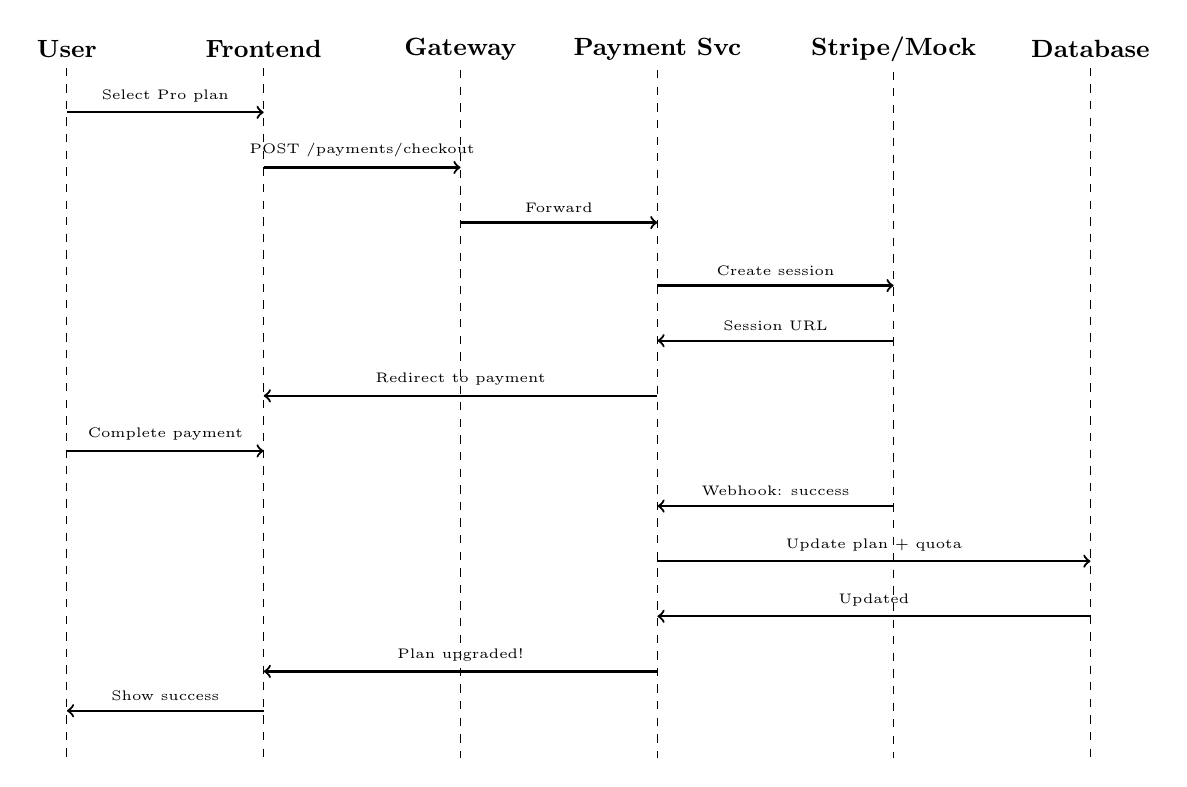
\begin{tikzpicture}[font=\small]
  \node (user) at (0, 0) {\textbf{User}};
  \node (front) at (2.5, 0) {\textbf{Frontend}};
  \node (gate) at (5, 0) {\textbf{Gateway}};
  \node (pay) at (7.5, 0) {\textbf{Payment Svc}};
  \node (stripe) at (10.5, 0) {\textbf{Stripe/Mock}};
  \node (db) at (13, 0) {\textbf{Database}};
  
  \draw[dashed] (user) -- (0, -9);
  \draw[dashed] (front) -- (2.5, -9);
  \draw[dashed] (gate) -- (5, -9);
  \draw[dashed] (pay) -- (7.5, -9);
  \draw[dashed] (stripe) -- (10.5, -9);
  \draw[dashed] (db) -- (13, -9);
  
  \draw[->, thick] (0, -0.8) -- node[above, font=\tiny] {Select Pro plan} (2.5, -0.8);
  \draw[->, thick] (2.5, -1.5) -- node[above, font=\tiny] {POST /payments/checkout} (5, -1.5);
  \draw[->, thick] (5, -2.2) -- node[above, font=\tiny] {Forward} (7.5, -2.2);
  \draw[->, thick] (7.5, -3) -- node[above, font=\tiny] {Create session} (10.5, -3);
  \draw[<-, thick] (7.5, -3.7) -- node[above, font=\tiny] {Session URL} (10.5, -3.7);
  \draw[<-, thick] (2.5, -4.4) -- node[above, font=\tiny] {Redirect to payment} (7.5, -4.4);
  \draw[->, thick] (0, -5.1) -- node[above, font=\tiny] {Complete payment} (2.5, -5.1);
  \draw[->, thick] (10.5, -5.8) -- node[above, font=\tiny] {Webhook: success} (7.5, -5.8);
  \draw[->, thick] (7.5, -6.5) -- node[above, font=\tiny] {Update plan + quota} (13, -6.5);
  \draw[<-, thick] (7.5, -7.2) -- node[above, font=\tiny] {Updated} (13, -7.2);
  \draw[<-, thick] (2.5, -7.9) -- node[above, font=\tiny] {Plan upgraded!} (7.5, -7.9);
  \draw[<-, thick] (0, -8.4) -- node[above, font=\tiny] {Show success} (2.5, -8.4);
\end{tikzpicture}
\caption{Sequence diagram — Plan upgrade with payment}
\label{fig:seq-payment}
\end{figure}

\subsection{Class Diagram — Payment Module}

\begin{figure}[H]
\centering
\begin{tikzpicture}[font=\small,
  class/.style={draw, rectangle, minimum width=3.5cm, align=left}
]
  \node[class, fill=yellow!15] (payment) at (0, 0) {
    \textbf{Payment}\\
    \hline
    - id: UUID\\
    - userId: UUID\\
    - planId: UUID\\
    - amount: Decimal\\
    - currency: String\\
    - status: PaymentStatus\\
    - stripeSessionId: String\\
    - createdAt: DateTime\\
    \hline
    + createCheckout()\\
    + processWebhook()
  };
  
  \node[class, fill=green!15] (pstatus) at (6, 0) {
    \textbf{<<enum>> PaymentStatus}\\
    \hline
    PENDING\\
    COMPLETED\\
    FAILED\\
    REFUNDED
  };
  
  \node[class, fill=blue!15] (invoice) at (0, -4.5) {
    \textbf{Invoice}\\
    \hline
    - id: UUID\\
    - paymentId: UUID\\
    - invoiceNumber: String\\
    - pdfUrl: String\\
    - createdAt: DateTime\\
    \hline
    + generate()
  };
  
  \draw[->, thick] (payment) -- (pstatus);
  \draw[->, thick] (payment) -- node[left, font=\tiny] {generates} (invoice);
\end{tikzpicture}
\caption{Class diagram — Payment module}
\label{fig:class-payment}
\end{figure}

\subsection{Implementation Screenshots}

\begin{figure}[H]
\centering
\fbox{\parbox{0.9\textwidth}{\centering\vspace{3cm}\textit{Insert billing page screenshot}\vspace{3cm}}}
\caption{Billing page — Current plan and usage}
\label{fig:billing-page}
\end{figure}

\begin{figure}[H]
\centering
\fbox{\parbox{0.9\textwidth}{\centering\vspace{3cm}\textit{Insert checkout flow screenshot}\vspace{3cm}}}
\caption{Checkout flow — Plan upgrade}
\label{fig:checkout}
\end{figure}

\begin{figure}[H]
\centering
\fbox{\parbox{0.9\textwidth}{\centering\vspace{3cm}\textit{Insert payment history screenshot}\vspace{3cm}}}
\caption{Payment history page}
\label{fig:payment-history}
\end{figure}

\subsection{Sprint 6 Review}

At the end of Sprint 6:
\begin{itemize}
  \item Payment service with plan CRUD and checkout.
  \item Stripe/mock payment processing with webhooks.
  \item Billing page displaying current plan and usage.
  \item Checkout flow for plan upgrades.
  \item Payment history with transaction records.
  \item Admin plan management page.
  \item SSL/TLS configured on the server.
\end{itemize}

% ============================================================
\section{Conclusion}

This chapter delivered the business layer of the platform. Sprint 5 enhanced the VM experience with detailed monitoring, \textbf{web-based CLI terminal access (Phase~1)}, and enforced resource limits through the quota system. Sprint 6 completed the monetization aspect with a full payment service supporting plan upgrades and billing history.

In the next chapter, we will finalize the platform with notifications, comprehensive testing, deployment, and project documentation.

% ============================================================
\chapter{Sprint 5 \& Sprint 6: Quotas and Payment Service}

\section{Introduction}

This chapter covers the business logic layer of the platform. Sprint 5 implements the VM dashboard with detailed information and the quota system that enforces resource limits per user. Sprint 6 delivers the payment service with plan management and upgrade flows.

% ============================================================
% SPRINT 5
% ============================================================
\section{Sprint 5: VM Dashboard \& Quota System}

\sprintcard{5}{VM Dashboard \& Quota System}{Deliver a comprehensive VM dashboard with status monitoring, and implement quota enforcement to limit resource usage per plan.}

\subsection{Sprint Backlog}

\begin{longtable}{|c|p{5cm}|c|c|c|}
\hline
\rowcolor{blue!15}
\textbf{Task ID} & \textbf{Task} & \textbf{Assignee} & \textbf{Est.} & \textbf{Status} \\
\hline
\endhead
T-5.1 & VM detail page (frontend) & DSI & 5h & Done \\
\hline
T-5.10 & Web terminal (xterm.js + WebSocket SSH) & DSI & 6h & Done \\
\hline
T-5.2 & VM action buttons + confirmation & DSI & 4h & Done \\
\hline
T-5.3 & Quota tracking implementation & DSI & 4h & Done \\
\hline
T-5.4 & Quota enforcement on VM creation & DSI & 3h & Done \\
\hline
T-5.5 & Admin VM management page & DSI & 5h & Done \\
\hline
T-5.6 & Quota display on dashboard & DSI & 3h & Done \\
\hline
T-5.7 & Server monitoring setup & RSI & 6h & Done \\
\hline
T-5.8 & Backup procedures & RSI & 4h & Done \\
\hline
T-5.9 & Network security audit & RSI & 4h & Done \\
\hline
\caption{Sprint 5 backlog}
\label{tab:sprint5-backlog}
\end{longtable}

\subsection{Use Case Diagram — Quota Management}

\begin{figure}[H]
\centering
\begin{tikzpicture}[
  usecase/.style={draw, ellipse, minimum width=3cm, minimum height=0.8cm, align=center, font=\scriptsize}
]
  \draw[thick, rounded corners] (0, -4.5) rectangle (7, 0.5);
  \node[font=\small\bfseries] at (3.5, 0.2) {Quota Management};
  
  \node (user) at (-2, -1.5) {User};
  \node (system) at (9.5, -2) {System};
  
  \node[usecase] (uc1) at (3.5, -0.5) {View Quota Usage};
  \node[usecase] (uc2) at (3.5, -1.5) {View Plan Details};
  \node[usecase] (uc3) at (3.5, -2.5) {Request VM Creation};
  \node[usecase] (uc4) at (3.5, -3.5) {Check Quota Limit};
  
  \draw (user) -- (uc1);
  \draw (user) -- (uc2);
  \draw (user) -- (uc3);
  \draw[dashed] (uc3) -- node[right, font=\tiny] {<<include>>} (uc4);
  \draw (system) -- (uc4);
\end{tikzpicture}
\caption{Use case diagram — Quota management}
\label{fig:uc-quota}
\end{figure}

\subsection{Sequence Diagram — Quota Check on VM Creation}

\begin{figure}[H]
\centering
\begin{tikzpicture}[font=\small]
  \node (user) at (0, 0) {\textbf{User}};
  \node (vmsvc) at (4, 0) {\textbf{VM Service}};
  \node (quota) at (8, 0) {\textbf{Quota Service}};
  \node (db) at (12, 0) {\textbf{Database}};
  
  \draw[dashed] (user) -- (0, -8);
  \draw[dashed] (vmsvc) -- (4, -8);
  \draw[dashed] (quota) -- (8, -8);
  \draw[dashed] (db) -- (12, -8);
  
  \draw[->, thick] (0, -1) -- node[above, font=\tiny] {Create VM request} (4, -1);
  \draw[->, thick] (4, -2) -- node[above, font=\tiny] {Check user quota} (8, -2);
  \draw[->, thick] (8, -3) -- node[above, font=\tiny] {Get user plan + VM count} (12, -3);
  \draw[<-, thick] (8, -3.5) -- node[above, font=\tiny] {Plan: Pro, VMs: 3/5} (12, -3.5);
  \draw[<-, thick] (4, -4.5) -- node[above, font=\tiny] {Quota OK (3 < 5)} (8, -4.5);
  \draw[->, thick] (4, -5.5) -- node[right, font=\tiny] {Proceed with creation};
  
  % Alternative (quota exceeded)
  \draw[thick, red, dashed] (1, -6) rectangle (11, -7.5);
  \node[red, font=\tiny] at (6, -6.3) {alt: Quota Exceeded};
  \draw[->, thick, red] (8, -7) -- node[above, font=\tiny, red] {403 Quota Exceeded} (4, -7);
\end{tikzpicture}
\caption{Sequence diagram — Quota check on VM creation}
\label{fig:seq-quota}
\end{figure}

\subsection{Class Diagram — Quota \& Plan}

\begin{figure}[H]
\centering
\begin{tikzpicture}[font=\small,
  class/.style={draw, rectangle, minimum width=3.5cm, align=left}
]
  \node[class, fill=yellow!15] (plan) at (0, 0) {
    \textbf{Plan}\\
    \hline
    - id: UUID\\
    - name: String\\
    - maxVMs: Integer\\
    - maxCPU: Integer\\
    - maxRAM: Integer\\
    - maxDisk: Integer\\
    - price: Decimal\\
    \hline
    + getPlans()
  };
  
  \node[class, fill=blue!15] (quota) at (6, 0) {
    \textbf{UserQuota}\\
    \hline
    - id: UUID\\
    - userId: UUID\\
    - planId: UUID\\
    - usedVMs: Integer\\
    - usedCPU: Integer\\
    - usedRAM: Integer\\
    - usedDisk: Integer\\
    \hline
    + checkLimit()\\
    + updateUsage()
  };
  
  \draw[->, thick] (quota) -- node[above, font=\tiny] {belongs to} (plan);
\end{tikzpicture}
\caption{Class diagram — Plan and quota}
\label{fig:class-quota}
\end{figure}

\subsection{Implementation Screenshots}

\begin{figure}[H]
\centering
\fbox{\parbox{0.9\textwidth}{\centering\vspace{3cm}\textit{Insert VM detail page screenshot}\vspace{3cm}}}
\caption{VM detail page with status, IP, and resources}
\label{fig:vm-detail}
\end{figure}

\begin{figure}[H]
\centering
\fbox{\parbox{0.9\textwidth}{\centering\vspace{3cm}\textit{Insert quota usage display screenshot}\vspace{3cm}}}
\caption{Dashboard — Quota usage display}
\label{fig:quota-display}
\end{figure}
\subsection{Sequence Diagram --- Web Terminal Connection}

\begin{figure}[H]
\centering
\begin{tikzpicture}[font=\small]
  \node (user) at (0, 0) {\textbf{User}};
  \node (front) at (3, 0) {\textbf{Frontend}};
  \node (gate) at (6, 0) {\textbf{Gateway}};
  \node (proxy) at (9, 0) {\textbf{SSH Proxy}};
  \node (vm) at (12, 0) {\textbf{VM (SSH)}};
  
  \draw[dashed] (user) -- (0, -9);
  \draw[dashed] (front) -- (3, -9);
  \draw[dashed] (gate) -- (6, -9);
  \draw[dashed] (proxy) -- (9, -9);
  \draw[dashed] (vm) -- (12, -9);
  
  \draw[->, thick] (0, -0.8) -- node[above, font=\tiny] {Click ``Terminal''} (3, -0.8);
  \draw[->, thick] (3, -1.5) -- node[above, font=\tiny] {WebSocket connect} (6, -1.5);
  \draw[->, thick] (6, -2.2) -- node[above, font=\tiny] {Get user SSH key} (6, -2.2);
  \draw[->, thick] (6, -2.7) -- node[right, font=\tiny] {Verify JWT};
  \draw[->, thick] (6, -3.5) -- node[above, font=\tiny] {Open SSH tunnel} (9, -3.5);
  \draw[->, thick] (9, -4.2) -- node[above, font=\tiny] {SSH connect (key auth)} (12, -4.2);
  \draw[<-, thick] (9, -4.9) -- node[above, font=\tiny] {Shell session open} (12, -4.9);
  \draw[<-, thick] (6, -5.6) -- node[above, font=\tiny] {Tunnel ready} (9, -5.6);
  \draw[<-, thick] (3, -6.3) -- node[above, font=\tiny] {WS connected} (6, -6.3);
  \draw[->, thick] (3, -7) -- node[below, font=\tiny] {xterm.js renders terminal} (3, -7);
  \draw[<->, thick] (0, -7.5) -- node[above, font=\tiny] {Type commands / see output} (3, -7.5);
  \draw[<->, thick, blue, dashed] (3, -8.2) -- node[above, font=\tiny, blue] {Bidirectional data stream} (12, -8.2);
\end{tikzpicture}
\caption{Sequence diagram --- Web terminal connection (Phase~1)}
\label{fig:seq-terminal}
\end{figure}

\begin{figure}[H]
\centering
\fbox{\parbox{0.9\textwidth}{\centering\vspace{3cm}\textit{Insert web terminal (CLI) screenshot --- user accessing VM from browser}\vspace{3cm}}}
\caption{Web terminal --- CLI access to VM via xterm.js (Phase~1)}
\label{fig:web-terminal}
\end{figure}
\subsection{Sprint 5 Review}

At the end of Sprint 5:
\begin{itemize}
  \item VM detail page showing IP, status, OS, CPU, RAM, uptime.
  \item \textbf{Web terminal (Phase~1)} --- users can access VMs via a CLI terminal in the browser using xterm.js and WebSocket SSH proxy.
  \item VM action buttons (start, stop, reboot, delete) with confirmation dialogs.
  \item Quota system tracking and enforcing resource limits.
  \item Admin VM management page with filtering.
  \item Server monitoring and backup procedures in place.
\end{itemize}


% ============================================================
% SPRINT 6
% ============================================================
\section{Sprint 6: Payment Service}

\sprintcard{6}{Payment Service}{Implement payment processing with plan management, upgrade flows, and billing history.}

\subsection{Sprint Backlog}

\begin{longtable}{|c|p{5cm}|c|c|c|}
\hline
\rowcolor{blue!15}
\textbf{Task ID} & \textbf{Task} & \textbf{Assignee} & \textbf{Est.} & \textbf{Status} \\
\hline
\endhead
T-6.1 & Plans CRUD (backend) & DSI & 4h & Done \\
\hline
T-6.2 & Payment processing (Stripe/mock) & DSI & 5h & Done \\
\hline
T-6.3 & Billing page (frontend) & DSI & 4h & Done \\
\hline
T-6.4 & Checkout flow (frontend) & DSI & 5h & Done \\
\hline
T-6.5 & Payment history page & DSI & 3h & Done \\
\hline
T-6.6 & Admin plan management page & DSI & 3h & Done \\
\hline
T-6.7 & SSL/TLS configuration & RSI & 4h & Done \\
\hline
T-6.8 & Log management & RSI & 4h & Done \\
\hline
T-6.9 & OpenNebula optimization & RSI & 4h & Done \\
\hline
\caption{Sprint 6 backlog}
\label{tab:sprint6-backlog}
\end{longtable}

\subsection{Use Case Diagram — Payment}

\begin{figure}[H]
\centering
\begin{tikzpicture}[
  usecase/.style={draw, ellipse, minimum width=3cm, minimum height=0.8cm, align=center, font=\scriptsize}
]
  \draw[thick, rounded corners] (0, -5.5) rectangle (7, 0.5);
  \node[font=\small\bfseries] at (3.5, 0.2) {Payment Module};
  
  \node (user) at (-2, -2) {User};
  \node (admin) at (9.5, -4) {Admin};
  
  \node[usecase] (uc1) at (3.5, -0.5) {View Current Plan};
  \node[usecase] (uc2) at (3.5, -1.5) {Compare Plans};
  \node[usecase] (uc3) at (3.5, -2.5) {Upgrade Plan};
  \node[usecase] (uc4) at (3.5, -3.5) {Process Payment};
  \node[usecase] (uc5) at (3.5, -4.5) {View Payment History};
  
  \draw (user) -- (uc1);
  \draw (user) -- (uc2);
  \draw (user) -- (uc3);
  \draw (user) -- (uc5);
  \draw[dashed] (uc3) -- node[right, font=\tiny] {<<include>>} (uc4);
  
  \node[usecase] (uc6) at (7.5, -5) {Manage Plans (CRUD)};
  \draw (admin) -- (uc6);
\end{tikzpicture}
\caption{Use case diagram — Payment module}
\label{fig:uc-payment}
\end{figure}

\subsection{Sequence Diagram — Plan Upgrade}

\begin{figure}[H]
\centering
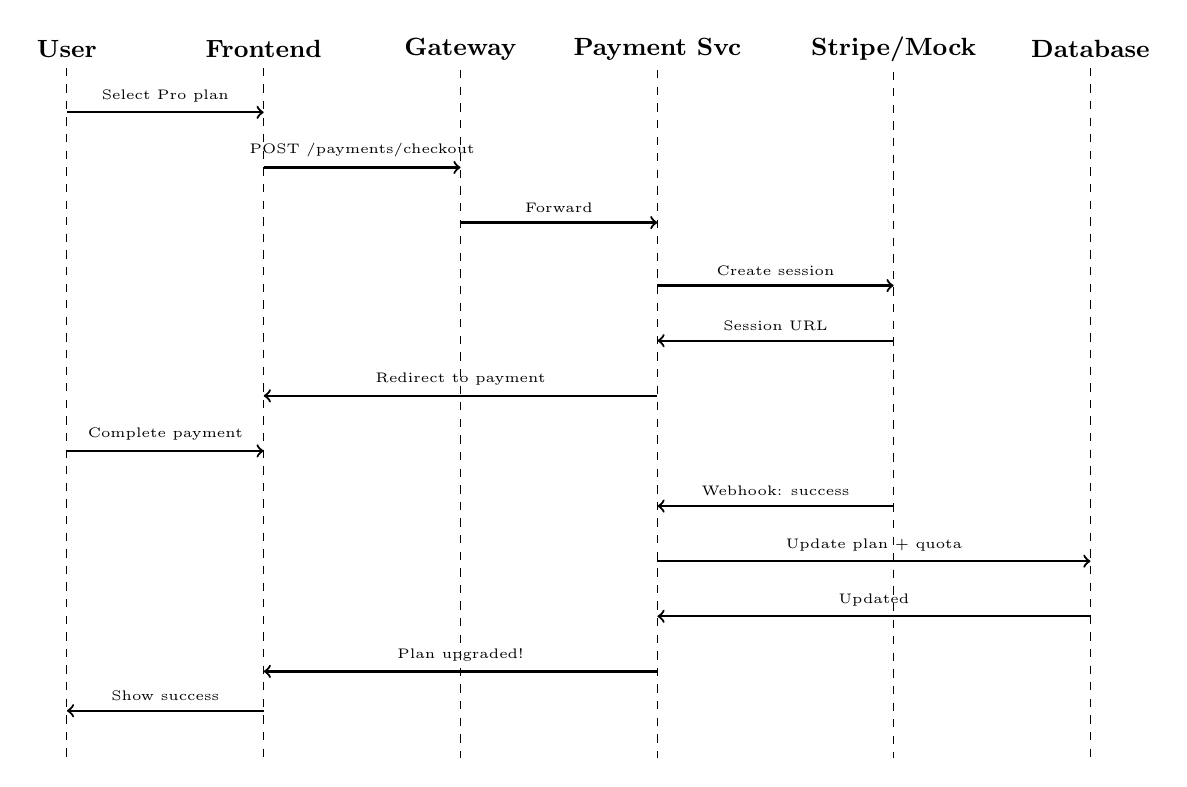
\begin{tikzpicture}[font=\small]
  \node (user) at (0, 0) {\textbf{User}};
  \node (front) at (2.5, 0) {\textbf{Frontend}};
  \node (gate) at (5, 0) {\textbf{Gateway}};
  \node (pay) at (7.5, 0) {\textbf{Payment Svc}};
  \node (stripe) at (10.5, 0) {\textbf{Stripe/Mock}};
  \node (db) at (13, 0) {\textbf{Database}};
  
  \draw[dashed] (user) -- (0, -9);
  \draw[dashed] (front) -- (2.5, -9);
  \draw[dashed] (gate) -- (5, -9);
  \draw[dashed] (pay) -- (7.5, -9);
  \draw[dashed] (stripe) -- (10.5, -9);
  \draw[dashed] (db) -- (13, -9);
  
  \draw[->, thick] (0, -0.8) -- node[above, font=\tiny] {Select Pro plan} (2.5, -0.8);
  \draw[->, thick] (2.5, -1.5) -- node[above, font=\tiny] {POST /payments/checkout} (5, -1.5);
  \draw[->, thick] (5, -2.2) -- node[above, font=\tiny] {Forward} (7.5, -2.2);
  \draw[->, thick] (7.5, -3) -- node[above, font=\tiny] {Create session} (10.5, -3);
  \draw[<-, thick] (7.5, -3.7) -- node[above, font=\tiny] {Session URL} (10.5, -3.7);
  \draw[<-, thick] (2.5, -4.4) -- node[above, font=\tiny] {Redirect to payment} (7.5, -4.4);
  \draw[->, thick] (0, -5.1) -- node[above, font=\tiny] {Complete payment} (2.5, -5.1);
  \draw[->, thick] (10.5, -5.8) -- node[above, font=\tiny] {Webhook: success} (7.5, -5.8);
  \draw[->, thick] (7.5, -6.5) -- node[above, font=\tiny] {Update plan + quota} (13, -6.5);
  \draw[<-, thick] (7.5, -7.2) -- node[above, font=\tiny] {Updated} (13, -7.2);
  \draw[<-, thick] (2.5, -7.9) -- node[above, font=\tiny] {Plan upgraded!} (7.5, -7.9);
  \draw[<-, thick] (0, -8.4) -- node[above, font=\tiny] {Show success} (2.5, -8.4);
\end{tikzpicture}
\caption{Sequence diagram — Plan upgrade with payment}
\label{fig:seq-payment}
\end{figure}

\subsection{Class Diagram — Payment Module}

\begin{figure}[H]
\centering
\begin{tikzpicture}[font=\small,
  class/.style={draw, rectangle, minimum width=3.5cm, align=left}
]
  \node[class, fill=yellow!15] (payment) at (0, 0) {
    \textbf{Payment}\\
    \hline
    - id: UUID\\
    - userId: UUID\\
    - planId: UUID\\
    - amount: Decimal\\
    - currency: String\\
    - status: PaymentStatus\\
    - stripeSessionId: String\\
    - createdAt: DateTime\\
    \hline
    + createCheckout()\\
    + processWebhook()
  };
  
  \node[class, fill=green!15] (pstatus) at (6, 0) {
    \textbf{<<enum>> PaymentStatus}\\
    \hline
    PENDING\\
    COMPLETED\\
    FAILED\\
    REFUNDED
  };
  
  \node[class, fill=blue!15] (invoice) at (0, -4.5) {
    \textbf{Invoice}\\
    \hline
    - id: UUID\\
    - paymentId: UUID\\
    - invoiceNumber: String\\
    - pdfUrl: String\\
    - createdAt: DateTime\\
    \hline
    + generate()
  };
  
  \draw[->, thick] (payment) -- (pstatus);
  \draw[->, thick] (payment) -- node[left, font=\tiny] {generates} (invoice);
\end{tikzpicture}
\caption{Class diagram — Payment module}
\label{fig:class-payment}
\end{figure}

\subsection{Implementation Screenshots}

\begin{figure}[H]
\centering
\fbox{\parbox{0.9\textwidth}{\centering\vspace{3cm}\textit{Insert billing page screenshot}\vspace{3cm}}}
\caption{Billing page — Current plan and usage}
\label{fig:billing-page}
\end{figure}

\begin{figure}[H]
\centering
\fbox{\parbox{0.9\textwidth}{\centering\vspace{3cm}\textit{Insert checkout flow screenshot}\vspace{3cm}}}
\caption{Checkout flow — Plan upgrade}
\label{fig:checkout}
\end{figure}

\begin{figure}[H]
\centering
\fbox{\parbox{0.9\textwidth}{\centering\vspace{3cm}\textit{Insert payment history screenshot}\vspace{3cm}}}
\caption{Payment history page}
\label{fig:payment-history}
\end{figure}

\subsection{Sprint 6 Review}

At the end of Sprint 6:
\begin{itemize}
  \item Payment service with plan CRUD and checkout.
  \item Stripe/mock payment processing with webhooks.
  \item Billing page displaying current plan and usage.
  \item Checkout flow for plan upgrades.
  \item Payment history with transaction records.
  \item Admin plan management page.
  \item SSL/TLS configured on the server.
\end{itemize}

% ============================================================
\section{Conclusion}

This chapter delivered the business layer of the platform. Sprint 5 enhanced the VM experience with detailed monitoring, \textbf{web-based CLI terminal access (Phase~1)}, and enforced resource limits through the quota system. Sprint 6 completed the monetization aspect with a full payment service supporting plan upgrades and billing history.

In the next chapter, we will finalize the platform with notifications, comprehensive testing, deployment, and project documentation.

% ============================================================
\chapter{Sprint 5 \& Sprint 6: Quotas and Payment Service}

\section{Introduction}

This chapter covers the business logic layer of the platform. Sprint 5 implements the VM dashboard with detailed information and the quota system that enforces resource limits per user. Sprint 6 delivers the payment service with plan management and upgrade flows.

% ============================================================
% SPRINT 5
% ============================================================
\section{Sprint 5: VM Dashboard \& Quota System}

\sprintcard{5}{VM Dashboard \& Quota System}{Deliver a comprehensive VM dashboard with status monitoring, and implement quota enforcement to limit resource usage per plan.}

\subsection{Sprint Backlog}

\begin{longtable}{|c|p{5cm}|c|c|c|}
\hline
\rowcolor{blue!15}
\textbf{Task ID} & \textbf{Task} & \textbf{Assignee} & \textbf{Est.} & \textbf{Status} \\
\hline
\endhead
T-5.1 & VM detail page (frontend) & DSI & 5h & Done \\
\hline
T-5.10 & Web terminal (xterm.js + WebSocket SSH) & DSI & 6h & Done \\
\hline
T-5.2 & VM action buttons + confirmation & DSI & 4h & Done \\
\hline
T-5.3 & Quota tracking implementation & DSI & 4h & Done \\
\hline
T-5.4 & Quota enforcement on VM creation & DSI & 3h & Done \\
\hline
T-5.5 & Admin VM management page & DSI & 5h & Done \\
\hline
T-5.6 & Quota display on dashboard & DSI & 3h & Done \\
\hline
T-5.7 & Server monitoring setup & RSI & 6h & Done \\
\hline
T-5.8 & Backup procedures & RSI & 4h & Done \\
\hline
T-5.9 & Network security audit & RSI & 4h & Done \\
\hline
\caption{Sprint 5 backlog}
\label{tab:sprint5-backlog}
\end{longtable}

\subsection{Use Case Diagram — Quota Management}

\begin{figure}[H]
\centering
\begin{tikzpicture}[
  usecase/.style={draw, ellipse, minimum width=3cm, minimum height=0.8cm, align=center, font=\scriptsize}
]
  \draw[thick, rounded corners] (0, -4.5) rectangle (7, 0.5);
  \node[font=\small\bfseries] at (3.5, 0.2) {Quota Management};
  
  \node (user) at (-2, -1.5) {User};
  \node (system) at (9.5, -2) {System};
  
  \node[usecase] (uc1) at (3.5, -0.5) {View Quota Usage};
  \node[usecase] (uc2) at (3.5, -1.5) {View Plan Details};
  \node[usecase] (uc3) at (3.5, -2.5) {Request VM Creation};
  \node[usecase] (uc4) at (3.5, -3.5) {Check Quota Limit};
  
  \draw (user) -- (uc1);
  \draw (user) -- (uc2);
  \draw (user) -- (uc3);
  \draw[dashed] (uc3) -- node[right, font=\tiny] {<<include>>} (uc4);
  \draw (system) -- (uc4);
\end{tikzpicture}
\caption{Use case diagram — Quota management}
\label{fig:uc-quota}
\end{figure}

\subsection{Sequence Diagram — Quota Check on VM Creation}

\begin{figure}[H]
\centering
\begin{tikzpicture}[font=\small]
  \node (user) at (0, 0) {\textbf{User}};
  \node (vmsvc) at (4, 0) {\textbf{VM Service}};
  \node (quota) at (8, 0) {\textbf{Quota Service}};
  \node (db) at (12, 0) {\textbf{Database}};
  
  \draw[dashed] (user) -- (0, -8);
  \draw[dashed] (vmsvc) -- (4, -8);
  \draw[dashed] (quota) -- (8, -8);
  \draw[dashed] (db) -- (12, -8);
  
  \draw[->, thick] (0, -1) -- node[above, font=\tiny] {Create VM request} (4, -1);
  \draw[->, thick] (4, -2) -- node[above, font=\tiny] {Check user quota} (8, -2);
  \draw[->, thick] (8, -3) -- node[above, font=\tiny] {Get user plan + VM count} (12, -3);
  \draw[<-, thick] (8, -3.5) -- node[above, font=\tiny] {Plan: Pro, VMs: 3/5} (12, -3.5);
  \draw[<-, thick] (4, -4.5) -- node[above, font=\tiny] {Quota OK (3 < 5)} (8, -4.5);
  \draw[->, thick] (4, -5.5) -- node[right, font=\tiny] {Proceed with creation};
  
  % Alternative (quota exceeded)
  \draw[thick, red, dashed] (1, -6) rectangle (11, -7.5);
  \node[red, font=\tiny] at (6, -6.3) {alt: Quota Exceeded};
  \draw[->, thick, red] (8, -7) -- node[above, font=\tiny, red] {403 Quota Exceeded} (4, -7);
\end{tikzpicture}
\caption{Sequence diagram — Quota check on VM creation}
\label{fig:seq-quota}
\end{figure}

\subsection{Class Diagram — Quota \& Plan}

\begin{figure}[H]
\centering
\begin{tikzpicture}[font=\small,
  class/.style={draw, rectangle, minimum width=3.5cm, align=left}
]
  \node[class, fill=yellow!15] (plan) at (0, 0) {
    \textbf{Plan}\\
    \hline
    - id: UUID\\
    - name: String\\
    - maxVMs: Integer\\
    - maxCPU: Integer\\
    - maxRAM: Integer\\
    - maxDisk: Integer\\
    - price: Decimal\\
    \hline
    + getPlans()
  };
  
  \node[class, fill=blue!15] (quota) at (6, 0) {
    \textbf{UserQuota}\\
    \hline
    - id: UUID\\
    - userId: UUID\\
    - planId: UUID\\
    - usedVMs: Integer\\
    - usedCPU: Integer\\
    - usedRAM: Integer\\
    - usedDisk: Integer\\
    \hline
    + checkLimit()\\
    + updateUsage()
  };
  
  \draw[->, thick] (quota) -- node[above, font=\tiny] {belongs to} (plan);
\end{tikzpicture}
\caption{Class diagram — Plan and quota}
\label{fig:class-quota}
\end{figure}

\subsection{Implementation Screenshots}

\begin{figure}[H]
\centering
\fbox{\parbox{0.9\textwidth}{\centering\vspace{3cm}\textit{Insert VM detail page screenshot}\vspace{3cm}}}
\caption{VM detail page with status, IP, and resources}
\label{fig:vm-detail}
\end{figure}

\begin{figure}[H]
\centering
\fbox{\parbox{0.9\textwidth}{\centering\vspace{3cm}\textit{Insert quota usage display screenshot}\vspace{3cm}}}
\caption{Dashboard — Quota usage display}
\label{fig:quota-display}
\end{figure}
\subsection{Sequence Diagram --- Web Terminal Connection}

\begin{figure}[H]
\centering
\begin{tikzpicture}[font=\small]
  \node (user) at (0, 0) {\textbf{User}};
  \node (front) at (3, 0) {\textbf{Frontend}};
  \node (gate) at (6, 0) {\textbf{Gateway}};
  \node (proxy) at (9, 0) {\textbf{SSH Proxy}};
  \node (vm) at (12, 0) {\textbf{VM (SSH)}};
  
  \draw[dashed] (user) -- (0, -9);
  \draw[dashed] (front) -- (3, -9);
  \draw[dashed] (gate) -- (6, -9);
  \draw[dashed] (proxy) -- (9, -9);
  \draw[dashed] (vm) -- (12, -9);
  
  \draw[->, thick] (0, -0.8) -- node[above, font=\tiny] {Click ``Terminal''} (3, -0.8);
  \draw[->, thick] (3, -1.5) -- node[above, font=\tiny] {WebSocket connect} (6, -1.5);
  \draw[->, thick] (6, -2.2) -- node[above, font=\tiny] {Get user SSH key} (6, -2.2);
  \draw[->, thick] (6, -2.7) -- node[right, font=\tiny] {Verify JWT};
  \draw[->, thick] (6, -3.5) -- node[above, font=\tiny] {Open SSH tunnel} (9, -3.5);
  \draw[->, thick] (9, -4.2) -- node[above, font=\tiny] {SSH connect (key auth)} (12, -4.2);
  \draw[<-, thick] (9, -4.9) -- node[above, font=\tiny] {Shell session open} (12, -4.9);
  \draw[<-, thick] (6, -5.6) -- node[above, font=\tiny] {Tunnel ready} (9, -5.6);
  \draw[<-, thick] (3, -6.3) -- node[above, font=\tiny] {WS connected} (6, -6.3);
  \draw[->, thick] (3, -7) -- node[below, font=\tiny] {xterm.js renders terminal} (3, -7);
  \draw[<->, thick] (0, -7.5) -- node[above, font=\tiny] {Type commands / see output} (3, -7.5);
  \draw[<->, thick, blue, dashed] (3, -8.2) -- node[above, font=\tiny, blue] {Bidirectional data stream} (12, -8.2);
\end{tikzpicture}
\caption{Sequence diagram --- Web terminal connection (Phase~1)}
\label{fig:seq-terminal}
\end{figure}

\begin{figure}[H]
\centering
\fbox{\parbox{0.9\textwidth}{\centering\vspace{3cm}\textit{Insert web terminal (CLI) screenshot --- user accessing VM from browser}\vspace{3cm}}}
\caption{Web terminal --- CLI access to VM via xterm.js (Phase~1)}
\label{fig:web-terminal}
\end{figure}
\subsection{Sprint 5 Review}

At the end of Sprint 5:
\begin{itemize}
  \item VM detail page showing IP, status, OS, CPU, RAM, uptime.
  \item \textbf{Web terminal (Phase~1)} --- users can access VMs via a CLI terminal in the browser using xterm.js and WebSocket SSH proxy.
  \item VM action buttons (start, stop, reboot, delete) with confirmation dialogs.
  \item Quota system tracking and enforcing resource limits.
  \item Admin VM management page with filtering.
  \item Server monitoring and backup procedures in place.
\end{itemize}


% ============================================================
% SPRINT 6
% ============================================================
\section{Sprint 6: Payment Service}

\sprintcard{6}{Payment Service}{Implement payment processing with plan management, upgrade flows, and billing history.}

\subsection{Sprint Backlog}

\begin{longtable}{|c|p{5cm}|c|c|c|}
\hline
\rowcolor{blue!15}
\textbf{Task ID} & \textbf{Task} & \textbf{Assignee} & \textbf{Est.} & \textbf{Status} \\
\hline
\endhead
T-6.1 & Plans CRUD (backend) & DSI & 4h & Done \\
\hline
T-6.2 & Payment processing (Stripe/mock) & DSI & 5h & Done \\
\hline
T-6.3 & Billing page (frontend) & DSI & 4h & Done \\
\hline
T-6.4 & Checkout flow (frontend) & DSI & 5h & Done \\
\hline
T-6.5 & Payment history page & DSI & 3h & Done \\
\hline
T-6.6 & Admin plan management page & DSI & 3h & Done \\
\hline
T-6.7 & SSL/TLS configuration & RSI & 4h & Done \\
\hline
T-6.8 & Log management & RSI & 4h & Done \\
\hline
T-6.9 & OpenNebula optimization & RSI & 4h & Done \\
\hline
\caption{Sprint 6 backlog}
\label{tab:sprint6-backlog}
\end{longtable}

\subsection{Use Case Diagram — Payment}

\begin{figure}[H]
\centering
\begin{tikzpicture}[
  usecase/.style={draw, ellipse, minimum width=3cm, minimum height=0.8cm, align=center, font=\scriptsize}
]
  \draw[thick, rounded corners] (0, -5.5) rectangle (7, 0.5);
  \node[font=\small\bfseries] at (3.5, 0.2) {Payment Module};
  
  \node (user) at (-2, -2) {User};
  \node (admin) at (9.5, -4) {Admin};
  
  \node[usecase] (uc1) at (3.5, -0.5) {View Current Plan};
  \node[usecase] (uc2) at (3.5, -1.5) {Compare Plans};
  \node[usecase] (uc3) at (3.5, -2.5) {Upgrade Plan};
  \node[usecase] (uc4) at (3.5, -3.5) {Process Payment};
  \node[usecase] (uc5) at (3.5, -4.5) {View Payment History};
  
  \draw (user) -- (uc1);
  \draw (user) -- (uc2);
  \draw (user) -- (uc3);
  \draw (user) -- (uc5);
  \draw[dashed] (uc3) -- node[right, font=\tiny] {<<include>>} (uc4);
  
  \node[usecase] (uc6) at (7.5, -5) {Manage Plans (CRUD)};
  \draw (admin) -- (uc6);
\end{tikzpicture}
\caption{Use case diagram — Payment module}
\label{fig:uc-payment}
\end{figure}

\subsection{Sequence Diagram — Plan Upgrade}

\begin{figure}[H]
\centering
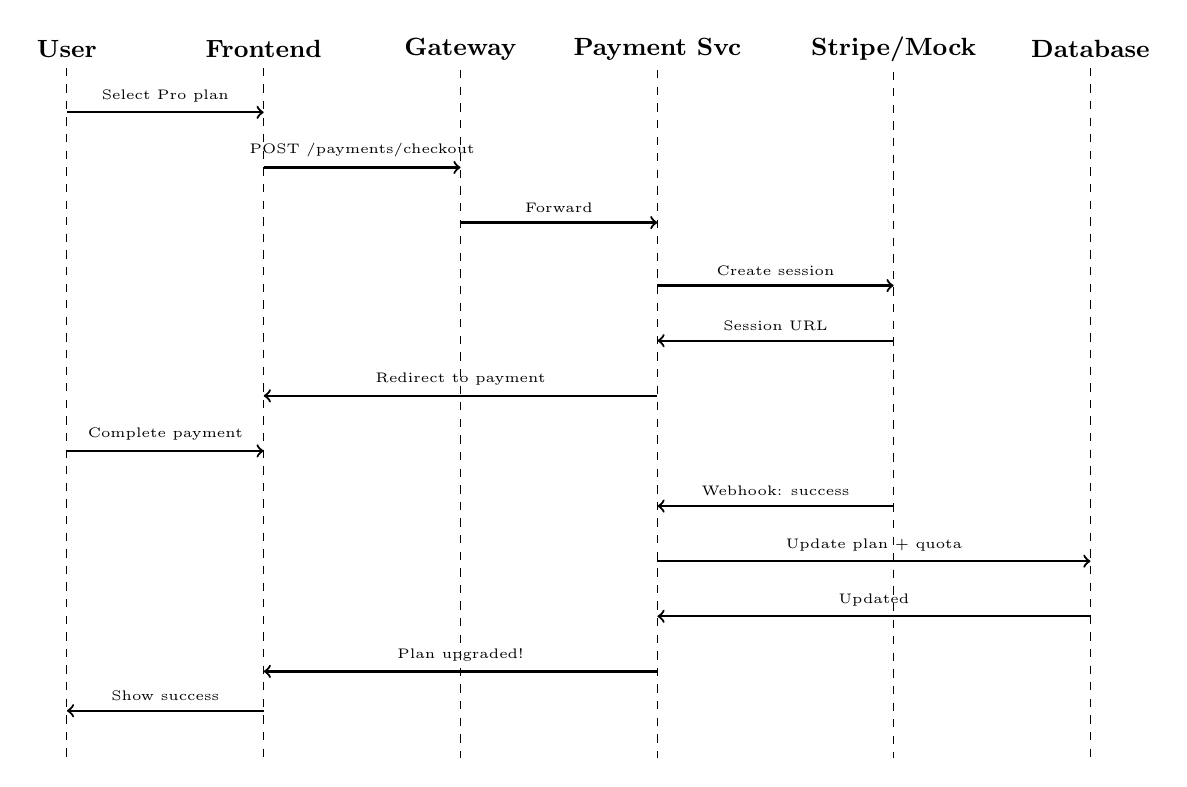
\begin{tikzpicture}[font=\small]
  \node (user) at (0, 0) {\textbf{User}};
  \node (front) at (2.5, 0) {\textbf{Frontend}};
  \node (gate) at (5, 0) {\textbf{Gateway}};
  \node (pay) at (7.5, 0) {\textbf{Payment Svc}};
  \node (stripe) at (10.5, 0) {\textbf{Stripe/Mock}};
  \node (db) at (13, 0) {\textbf{Database}};
  
  \draw[dashed] (user) -- (0, -9);
  \draw[dashed] (front) -- (2.5, -9);
  \draw[dashed] (gate) -- (5, -9);
  \draw[dashed] (pay) -- (7.5, -9);
  \draw[dashed] (stripe) -- (10.5, -9);
  \draw[dashed] (db) -- (13, -9);
  
  \draw[->, thick] (0, -0.8) -- node[above, font=\tiny] {Select Pro plan} (2.5, -0.8);
  \draw[->, thick] (2.5, -1.5) -- node[above, font=\tiny] {POST /payments/checkout} (5, -1.5);
  \draw[->, thick] (5, -2.2) -- node[above, font=\tiny] {Forward} (7.5, -2.2);
  \draw[->, thick] (7.5, -3) -- node[above, font=\tiny] {Create session} (10.5, -3);
  \draw[<-, thick] (7.5, -3.7) -- node[above, font=\tiny] {Session URL} (10.5, -3.7);
  \draw[<-, thick] (2.5, -4.4) -- node[above, font=\tiny] {Redirect to payment} (7.5, -4.4);
  \draw[->, thick] (0, -5.1) -- node[above, font=\tiny] {Complete payment} (2.5, -5.1);
  \draw[->, thick] (10.5, -5.8) -- node[above, font=\tiny] {Webhook: success} (7.5, -5.8);
  \draw[->, thick] (7.5, -6.5) -- node[above, font=\tiny] {Update plan + quota} (13, -6.5);
  \draw[<-, thick] (7.5, -7.2) -- node[above, font=\tiny] {Updated} (13, -7.2);
  \draw[<-, thick] (2.5, -7.9) -- node[above, font=\tiny] {Plan upgraded!} (7.5, -7.9);
  \draw[<-, thick] (0, -8.4) -- node[above, font=\tiny] {Show success} (2.5, -8.4);
\end{tikzpicture}
\caption{Sequence diagram — Plan upgrade with payment}
\label{fig:seq-payment}
\end{figure}

\subsection{Class Diagram — Payment Module}

\begin{figure}[H]
\centering
\begin{tikzpicture}[font=\small,
  class/.style={draw, rectangle, minimum width=3.5cm, align=left}
]
  \node[class, fill=yellow!15] (payment) at (0, 0) {
    \textbf{Payment}\\
    \hline
    - id: UUID\\
    - userId: UUID\\
    - planId: UUID\\
    - amount: Decimal\\
    - currency: String\\
    - status: PaymentStatus\\
    - stripeSessionId: String\\
    - createdAt: DateTime\\
    \hline
    + createCheckout()\\
    + processWebhook()
  };
  
  \node[class, fill=green!15] (pstatus) at (6, 0) {
    \textbf{<<enum>> PaymentStatus}\\
    \hline
    PENDING\\
    COMPLETED\\
    FAILED\\
    REFUNDED
  };
  
  \node[class, fill=blue!15] (invoice) at (0, -4.5) {
    \textbf{Invoice}\\
    \hline
    - id: UUID\\
    - paymentId: UUID\\
    - invoiceNumber: String\\
    - pdfUrl: String\\
    - createdAt: DateTime\\
    \hline
    + generate()
  };
  
  \draw[->, thick] (payment) -- (pstatus);
  \draw[->, thick] (payment) -- node[left, font=\tiny] {generates} (invoice);
\end{tikzpicture}
\caption{Class diagram — Payment module}
\label{fig:class-payment}
\end{figure}

\subsection{Implementation Screenshots}

\begin{figure}[H]
\centering
\fbox{\parbox{0.9\textwidth}{\centering\vspace{3cm}\textit{Insert billing page screenshot}\vspace{3cm}}}
\caption{Billing page — Current plan and usage}
\label{fig:billing-page}
\end{figure}

\begin{figure}[H]
\centering
\fbox{\parbox{0.9\textwidth}{\centering\vspace{3cm}\textit{Insert checkout flow screenshot}\vspace{3cm}}}
\caption{Checkout flow — Plan upgrade}
\label{fig:checkout}
\end{figure}

\begin{figure}[H]
\centering
\fbox{\parbox{0.9\textwidth}{\centering\vspace{3cm}\textit{Insert payment history screenshot}\vspace{3cm}}}
\caption{Payment history page}
\label{fig:payment-history}
\end{figure}

\subsection{Sprint 6 Review}

At the end of Sprint 6:
\begin{itemize}
  \item Payment service with plan CRUD and checkout.
  \item Stripe/mock payment processing with webhooks.
  \item Billing page displaying current plan and usage.
  \item Checkout flow for plan upgrades.
  \item Payment history with transaction records.
  \item Admin plan management page.
  \item SSL/TLS configured on the server.
\end{itemize}

% ============================================================
\section{Conclusion}

This chapter delivered the business layer of the platform. Sprint 5 enhanced the VM experience with detailed monitoring, \textbf{web-based CLI terminal access (Phase~1)}, and enforced resource limits through the quota system. Sprint 6 completed the monetization aspect with a full payment service supporting plan upgrades and billing history.

In the next chapter, we will finalize the platform with notifications, comprehensive testing, deployment, and project documentation.
